\documentclass{jsarticle}

\title{
    コズミックトラベル \\
    \large 75th2600内装設計チーフ引き継ぎ
}
\author{75th621 千葉森生}
\date{最終更新日: \today}

\usepackage[dvipdfmx]{graphicx}
\usepackage{subcaption}
\usepackage[dvipdfmx,hidelinks]{hyperref}
\usepackage{pxjahyper}

\newcommand*{\includefig}[5][c]{%
    \begin{minipage}[#1]{#2\linewidth}
        \centering
        \includegraphics[width=\linewidth]{#5}
        \subcaption{#3}
        \label{#4}
    \end{minipage}
}
\newenvironment{imageHere}[2][htbp]{\def\@imageHereTmp{#2}%
    \begin{figure}[#1]
        \centering
}{%  
        \caption{\@imageHereTmp}
        \label{fig:\@imageHereTmp}
    \end{figure}
}

\begin{document}

\maketitle

\section{まえがき}

入試を間近に控えておきながら今更2年生の引き継ぎを書いているのは、3年のはいいから2年の時の引き継ぎをかけと急かされている私、内設チのライド担当の千葉でございます。

軽くプロフィール(肩書き自慢)を書くと、以下のようになります。
\begin{itemize}
    \item 75th2600, 3600内装設計チーフ
    \item 75th2600原案班
    \item エンジニアチームCTO
    \item 帰宅部 etc...
\end{itemize}

で、どんな内装を作ったかと言いますと、

\begin{imageHere}{設計概観}
    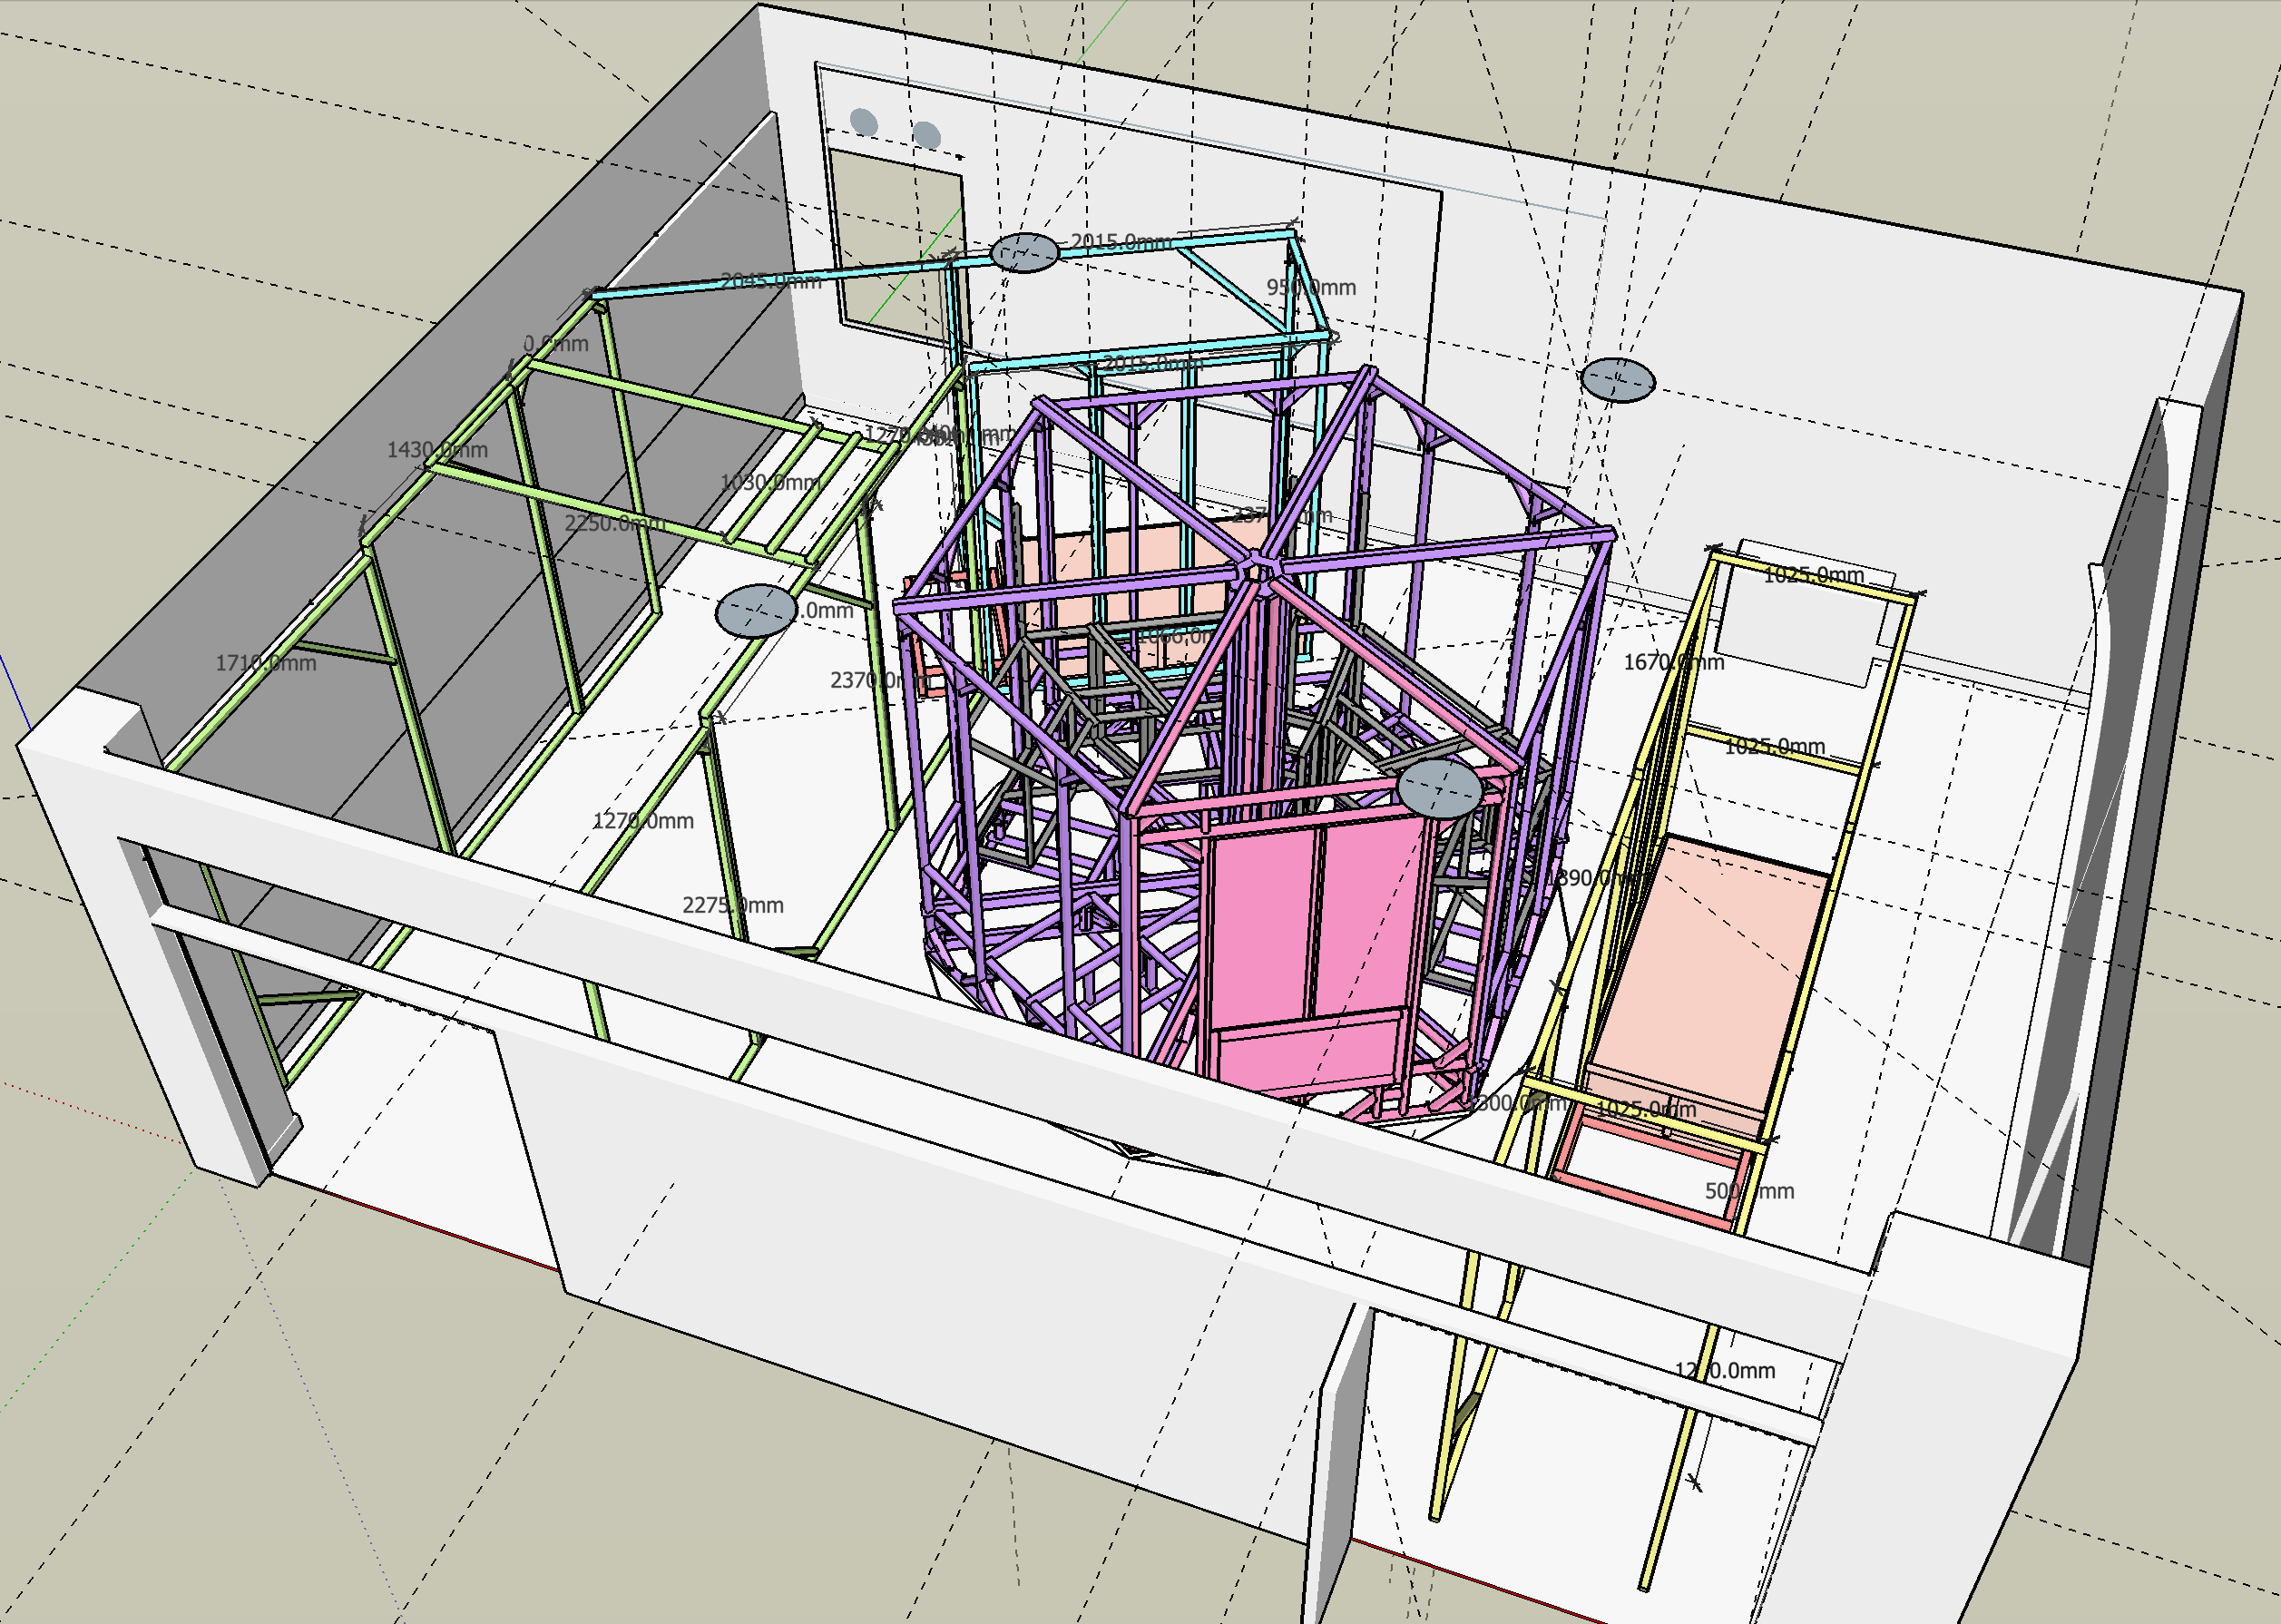
\includegraphics[width=0.5\linewidth]{images/plan_overview/1.png}
\end{imageHere}

こんなのです。真ん中の正六角形の宇宙船に人を2,3人乗せて回しました。そのため、その辺りの補強が割とエグいです。
今後ライドをやるクラスの参考になれば幸いです。
なお、設計チーフの身ながら内チの仕事に近いところまで手を伸ばしていたので、割と手広い引き継ぎになってます。

デザインが論文っぽいのは\LaTeX{}で書いてるからです。あと、資料は全部別ファイルで添付して、一部のみ引用してきてます。詳しく見たければ添付ファイルへgo。

\clearpage

\tableofcontents

\section{TL;DR}
TL;DRってIT界隈でしか通じないらしいですね。Too Long, Don't Readの略で、要約みたいな意味のスラングです。

で、要約、というか伝えたいこと。主に心構え的なこととか。

\begin{itemize}
    \item デザインを待っていたら設計は終わらない。設チが先導せよ。
    \item 目標は高くもて。ただし周りのアドバイスは聞け。
    \item 外装との連携は忘れずに。双方の進捗を見て人員とか作業スペースとか融通しよう。
    \item 教室測定は念入りに。正確に。細部まで。
\end{itemize}

あと、引き継ぎの内容についてでもそれ以外でも、何か質問があればこちらのメールアドレスまでお気軽に:  chibam496@gmail.com

\clearpage

\section{概要}
\subsection{成果物}

まずは作ったものの紹介から。

\begin{imageHere}{骨組み}
    \includefig{0.45}{完成形}{fig:完成形}{images/plan_overview/2.jpg}
    \includefig{0.45}{完成直前}{fig:完成直前}{images/plan_overview/3.jpg}
\end{imageHere}

正三角形のパーツを6個作り、ネジで繋ぎ合わせて作りました。後述しますが、分割して組み立てる方法は教室復元\footnote{\hyperlink{note:教室復元}{p.7の脚注}を参照}を意識したものなので、似たようなのを作る場合は分割せずまとめて作ってしまうのもありかと思います。
特徴としては、稼働部が巨大であること、それに応じて補強も複雑であることです。


\begin{imageHere}{装飾後}
    \begin{minipage}{0.45\linewidth}
        \centering
        \includefig{1}{宇宙船の内装}{fig:内装}{images/plan_overview/4.jpg}
        \includefig{1}{降りた後の通路から出口方面}{fig:出口}{images/plan_overview/5.jpg}
    \end{minipage}\hfill
    \begin{minipage}{0.45\linewidth}
        \centering
        \includefig{1}{ライドを動かす様子}{fig:人力}{images/plan_overview/6.jpg}
    \end{minipage}
\end{imageHere}

基本的に二人乗りですが、動き回ることを想定しているので実際は5人ぐらい入っても問題ない大きさ。もっとも、ライドを回すのは人力なので、あまり重いと回りませんが。

\clearpage

\subsection{動線}

\begin{imageHere}{動線}
    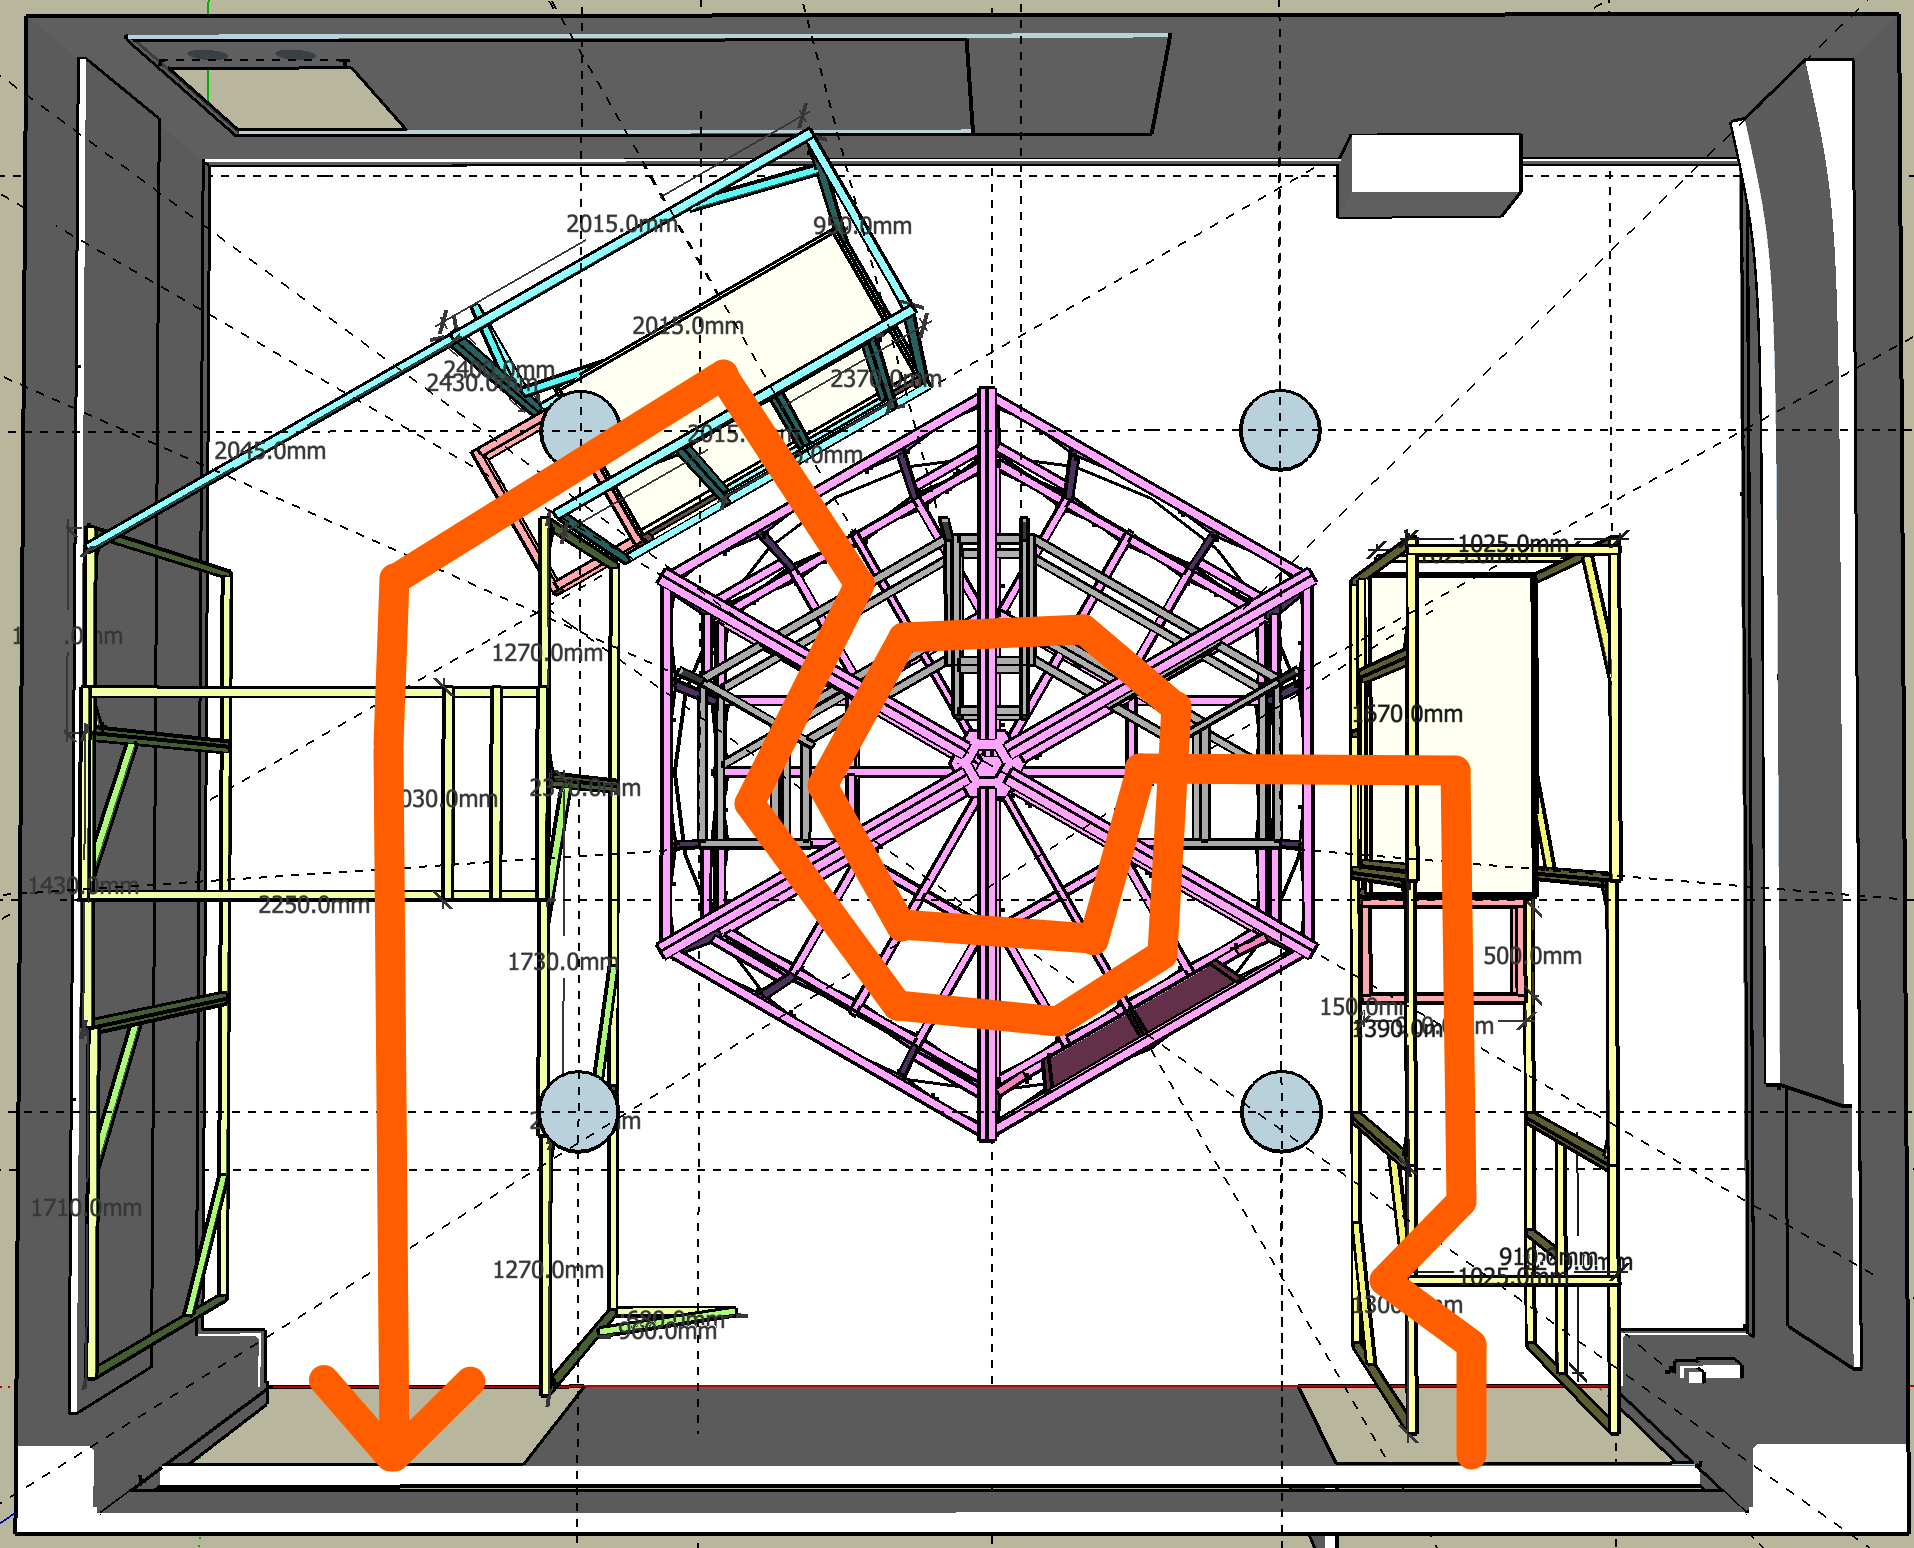
\includegraphics[width=0.6\linewidth]{images/plan_overview/lane.png}
\end{imageHere}

\begin{enumerate}
    \item 教室前方のドアが入り口、入って左側に受付
    \item そのまま進み、渡し板を渡って宇宙船に乗り込む
    \item ミニゲームを解く間に、ストーリーに合わせて宇宙船が回転
    \item 宇宙船から降りた後、出口側の通路でミニゲームの結果に応じた映像を流す
    \item 教室後方から出て終了
\end{enumerate}

\clearpage

\section{案の確定に至るまで}

\subsection{第1回プレゼン大会@Jan 13 (原案班)}

我々のクラスでは、数人ずつのグループを作って案を考え、2回のプレゼンを経て最終案を決定しました。

初期の案では、4組が同時に参加できる方式を考えていました。4つの少しずつ異なる部屋を用意して相互に連結し、レールの上を回す、というアイデアです。
ミニゲームについては具体的に決めず、クラスから公募する方針でした。
この段階で、プレゼンに向けてBlenderを用いて3Dモデルを作成しました。
具体的なサイズなどが感覚的にわかるため、これはかなり良かったです。sketchupでも構わないので作るといいと思います。

\begin{imageHere}{原案1}
    \includefig{0.45}{企画書}{fig:企画書}{images/presentation/original_plan.png}
    \includefig{0.45}{3Dモデル}{fig:3Dモデル1}{images/presentation/3D_model/3D_model_1_1.png}
\end{imageHere}

\clearpage

\subsection{第2回プレゼン大会@Feb 10 (原案班)}

十分な耐久性、安定性のあるレールが低コストでは作れない、連結部の耐久性が確保できないなどの理由から、レールを用いた方式を取り止めました。
代わりに採用したのが、成蹊大学の「劇団円想者」\footnote{\url{http://yensosha.blog53.fc2.com/blog-entry-592.html}}がブログに写真を公開していた回り舞台です。この構造なら全て一体型のため連結部やレールが不要で、キャスターのみで回すことができます。
骨組みの基本的な構造は、最後までこれを踏襲しています。
6つのパーツに分かれているため文化祭前の教室復元
    \footnote{\hypertarget{note:教室復元}{教室復元}とは、夏休みと文化祭の間に授業日があったため、そこに向けて内装を一旦解体するイベント。コロナ禍のため平時以上に広いスペースを確保しなければならなかった。幸い、この年の教室復元は最終的になくなり、翌2022年もなかった。今後も復活することはないと思われる。}
でパーツに分けて教室の隅に寄せることができる、補強さえすれば余計なコストをかけずに木材だけで十分な強度が得られることなどが採用理由です。

\begin{imageHere}{原案2-1}
    \begin{minipage}{0.5\linewidth}
        \centering
        \includefig{1}{3Dモデル}{fig:3Dモデル2}{images/presentation/3D_model/3D_model_2_2.png}
    \end{minipage}\hfill
    \begin{minipage}{0.4\linewidth}
        \centering
        \includefig{1}{円想者の舞台(1)}{fig:円想者1}{images/presentation/base_bone_1.jpg}
        \includefig{1}{円想者の舞台(2)}{fig:円想者2}{images/presentation/base_bone_2.jpg}
    \end{minipage}
\end{imageHere}

\begin{imageHere}{原案2-2}
    \includefig{0.45}{スライドの抜粋(1)}{fig:スライド1}{images/presentation/presentation2_1.png}
    \includefig{0.45}{スライドの抜粋(2)}{fig:スライド2}{images/presentation/presentation2_2.png}
    \includefig{0.35}{ミニゲームについて}{fig:ミニゲーム}{images/presentation/minigame.jpg}
    \includefig{0.25}{意見・質問(1)}{fig:質問1}{images/presentation/feedback_1.png}
    \includefig{0.25}{意見・質問(2)}{fig:質問2}{images/presentation/feedback_2.png}
    \includefig{0.45}{意見・質問への解答}{fig:質問3}{images/presentation/feedback_3.png}
\end{imageHere}

\clearpage

\subsection{展示決定@Mar 3}

上記の案で確定し、ストーリーやミニゲームなどの詳細を作り始めました。

このころ、部屋を分けることで無駄な空間が多くなり、各部屋がかなり狭くなってしまうことが判明し、\\一つの箱を2または3個に分割する案に移行しました。

\begin{imageHere}{部屋の分割}
    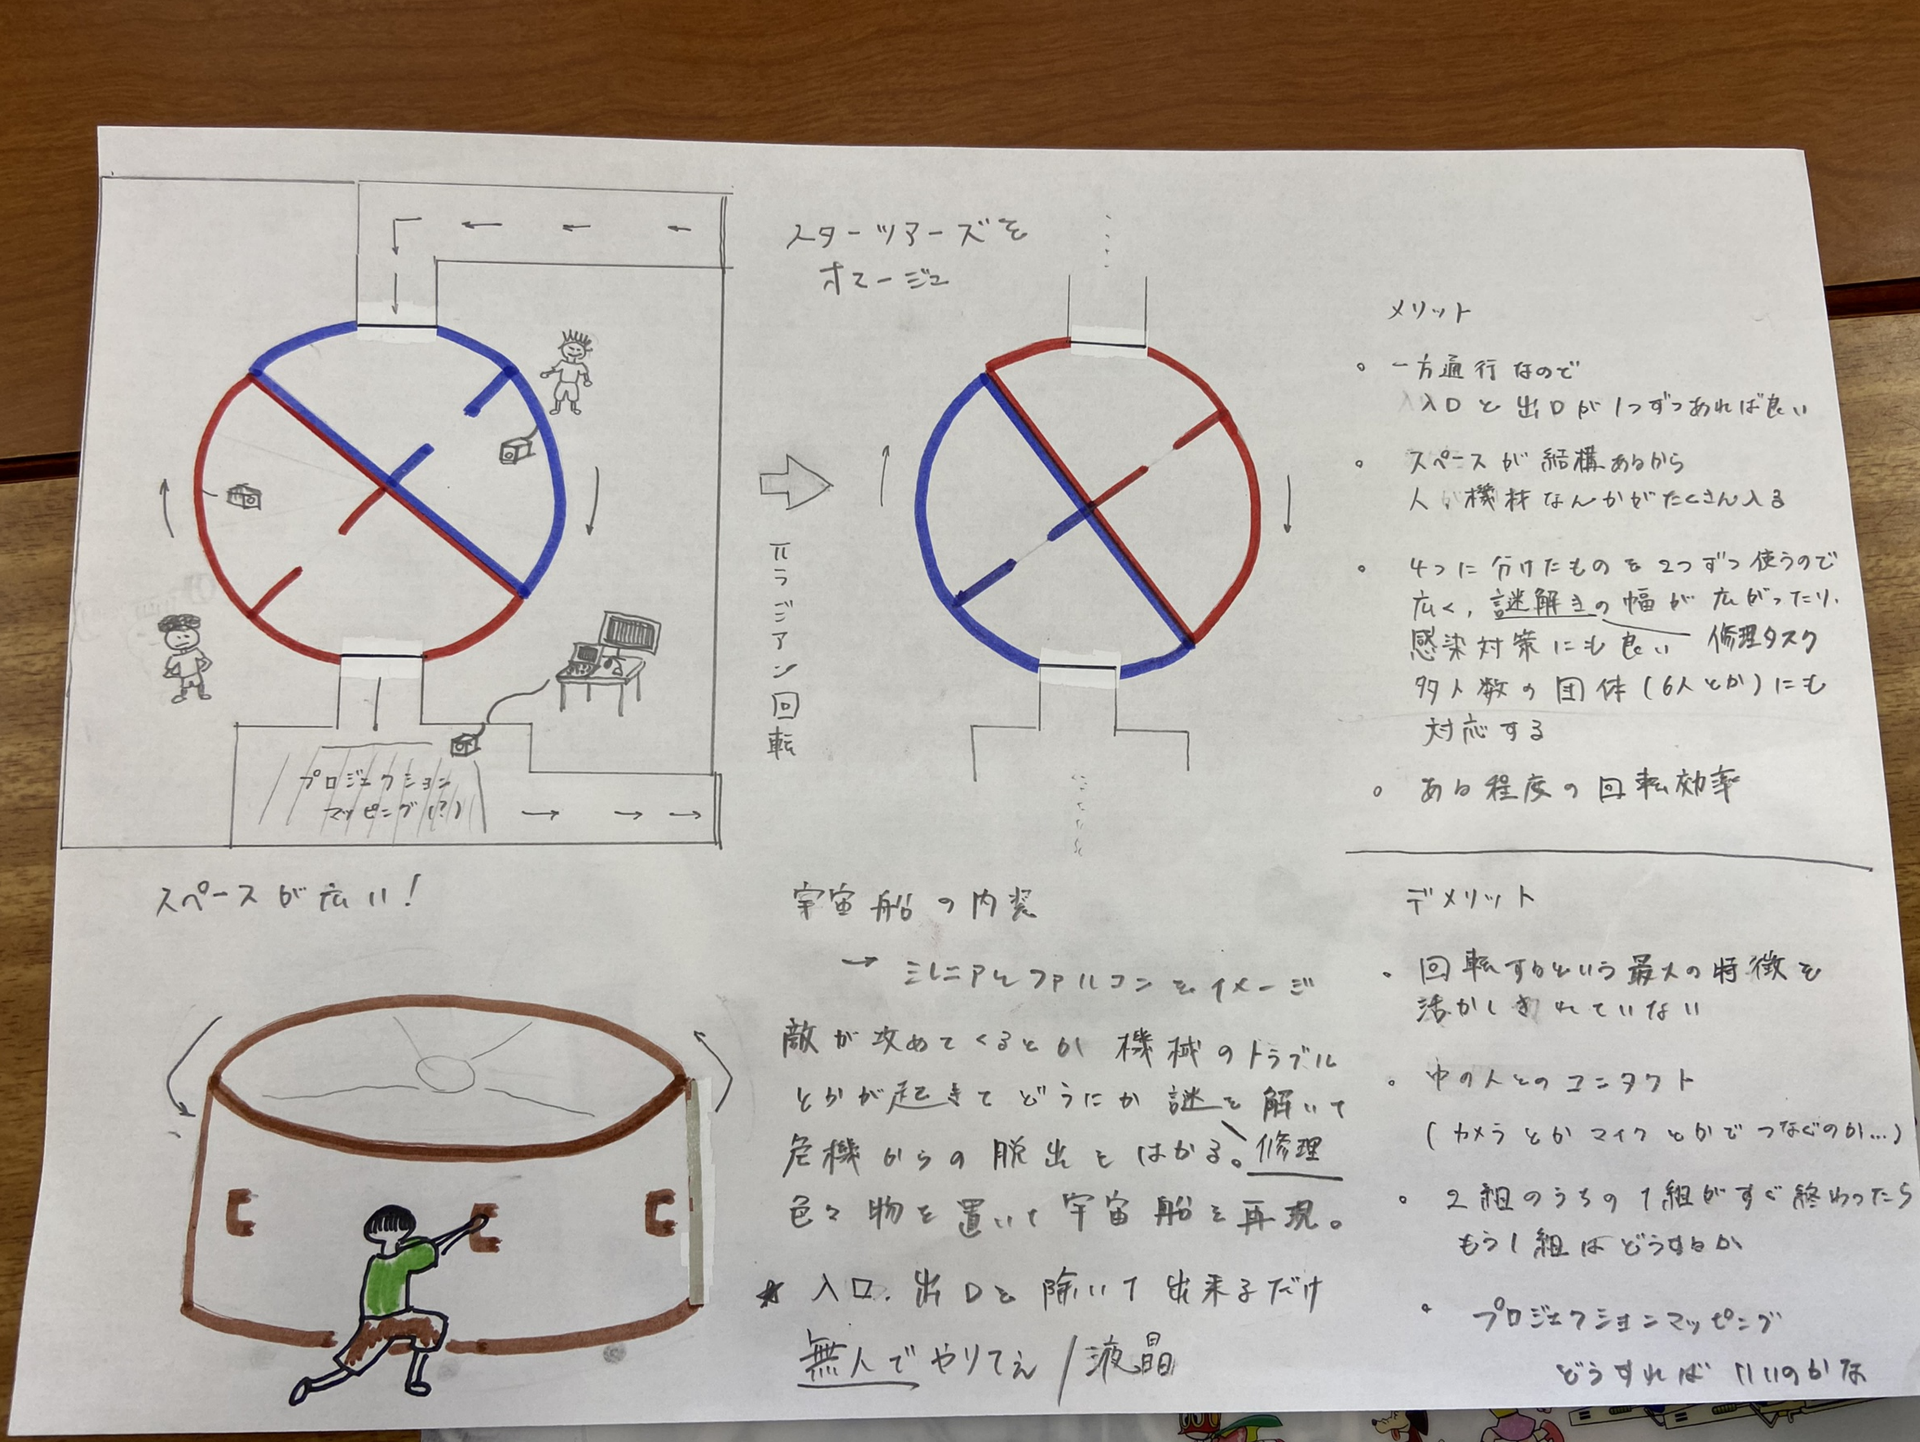
\includegraphics[width=0.7\linewidth]{images/minigame/0.png}
\end{imageHere}

\subsection{ミニゲームプレゼン@Mar 22}

具体的なゲーム内容を決定します。これによって細部の設計、例えば宇宙船外にも構造を作る必要があるのか、タラップの構造はどうするのか、などが決まってきます。
また、デザイン案についても具体的なものが多く出てきたので、ここから本格的な設計の検討が始まりました。

6案が出て、そのうち佐野案(図\ref{figs:ミニゲームプレゼン}\subref{fig:佐野案})では紙で内装の模型(図\ref{figs:ミニゲームプレゼン}\subref{fig:模型1}\subref{fig:模型2})を作ってきてくれました。
実際に宇宙船が回転できるものだったので皆にイメージを持ってもらうためにも一役買い、最後までお世話になった模型になりました。
また、同案の内装のイメージはそのままの再現こそできなかったもの、ドアなどのデザイン・設計の目標となりました。

田中案(図\ref{figs:ミニゲームプレゼン}\subref{fig:田中案})は最終的なストーリーのベースとなりました。
ただ、船外の装飾は時間的制約の関係で実現できず、窓も無くなっています。

\begin{imageHere}{ミニゲームプレゼン}
    \includefig[t]{0.45}{模型-全体像}{fig:模型1}{images/minigame/1.jpg}
    \vspace{-35mm}
    \includefig[c]{0.45}{模型-タラップ}{fig:模型2}{images/minigame/2.jpg}
    \includefig[b]{0.45}{内装イメージ(佐野案)}{fig:佐野案}{images/minigame/3.jpg}
    \includefig[b]{0.45}{船外を装飾する案(田中案)}{fig:田中案}{images/minigame/4.jpg}
\end{imageHere}

\clearpage

\subsection{デザイン開始@May 30}
まずはタラップからデザインが開始しました。なお、設計はとっくに始まっていて、内チに催促しまくってデザイン班を動かしてもらいました。
デザインが完成するのはどうしてもぎりぎりになりがちです。デザインを待ってから設計するという考えは抱かず、後から修正すればいいと思ってどんどん突き進んでしまいましょう。

ちなみにこの段階の設計は、まだsketchupでは作らず、ひたすらに教室の測定と黒板を用いた平面図での設計をもう一人の内設チと一緒に行っていました。緊急時の通路などをふくめゲストの通る可能性のある場所がもれなく文実規則を満たすようにしなければならず、特に宇宙船と壁の間の間隔を確保するための計算が面倒くさかったです。

それから、板パタと書いてあるやつは宇宙船とタラップの間の渡り板のことで、紆余曲折あって最終的に「イカ」と呼ばれるようになっていきます。

\begin{imageHere}{平面図}
    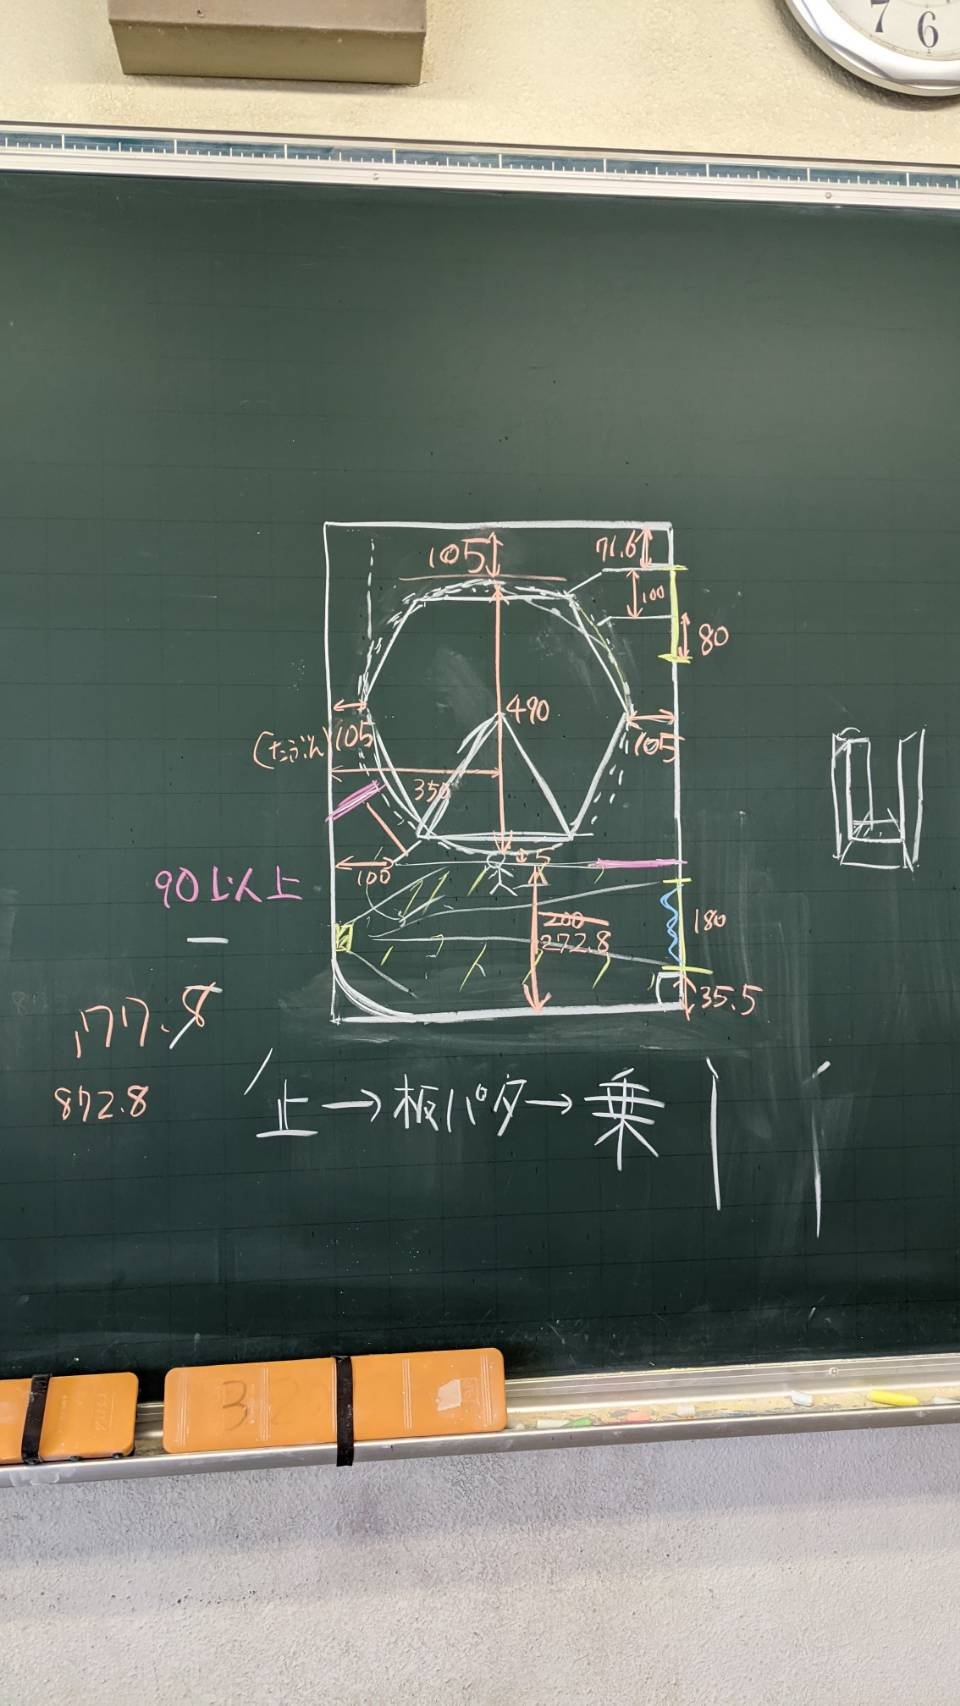
\includegraphics[width=0.45\linewidth]{images/plan/69138.jpg}
\end{imageHere}

\clearpage

\section{骨組みについて}

いよいよ本題ですね。実際に

\end{document}